\documentclass[11pt,a4paper]{article}

\usepackage[left=2cm,text={17cm,24cm},top=3cm]{geometry}
\usepackage[bookmarksopen,colorlinks,plainpages=false,urlcolor=blue,unicode,linkcolor=blue]{hyperref}
\usepackage[slovak]{babel}
\usepackage[utf8]{inputenc}
\usepackage[T1]{fontenc}
\usepackage{indentfirst}
\usepackage{graphicx}
\usepackage{eurosym}
\usepackage{float}
\usepackage{url}

\graphicspath{{.}}

\begin{document}

% #################################################################################################
% TITLEPAGE

\begin{titlepage}
    \begin{center}
        \Huge
        \textsc{
            Fakulta informačních technologií\\
            Vysoké učení technické v~Brně
        }
        \vspace{100px}
        \begin{figure}[!h]
            \centering
            
\includegraphics[scale=0.3]{img/vutbr-fit-logo.eps}
        \end{figure}
        \\[25mm]
        \huge{
            \textbf{
                Odvoz komunálneho odpadu v meste\\
                Rimavská Sobota
            }
        }
        \vfill
    \end{center}
        \Large{
            \hfill\\
            Peter Šuhaj (xsuhaj02)\\
            Adrián Tóth (xtotha01) \hfill \today
        }

\end{titlepage}

% #################################################################################################
% CONTENT

\setlength{\parskip}{0pt}
\hypersetup{hidelinks}\tableofcontents
\setlength{\parskip}{0pt}

\newpage %#########################################################################################

\section{Úvod}

    \indent Táto práca sa zoberá problematikou odvozu komunálneho odpadu v meste Rimavská Sobota v Slovenskej republike. Pre daný problém bol navrhnutý a implementovaný model - \cite{IMS}(str. č. 7), ktorý sa využíva na simulačné účely - \cite{IMS}(str. č. 8). Simulačné výsledky slúžia na získavanie poznatkov o odvoze komunálneho odpadu, ktoré budú skúmané a popísane v ďalších kapitolách.\\[0.4em]
    \indent Cieľom práce je poukázať na fakty ktoré môžu odvoz komunálneho odpadu ovplivniť z ekonomického hľadiska. Zmysel tejto práce je nájsť čo najekonomickejšie riešenie na náklady odvozu odpadu v meste Rimavská Sobota.

    \subsection{Zadanie}

        \indent Zadanie tejto práce spadalo do časti \textit{služby, infrastruktura a energetika}\cite{IMS-TEMA} pod číslom \textit{5}, ktoré nám bolo náhodne pridelené. Vybrali sme si problematiku \textit{odpadové hospodárstvo} z oblasti \textit{infraštruktúry}.

    \subsection{Autori a zdroje}

        \indent Autormi tohto projektu sú Peter Šuhaj (xsuhaj02) a Adrián Tóth (xtotha01) - študenti 3. ročníka bakalárskeho štúdia na \textit{Fakultě informačních technologií - Vysokého učení technického v Brně}\cite{VUT-FIT}.\\[0.4em]
        \indent Zdroje informácii potrebné k vypracovaniu projektu boli získané od pána Attilu Šimka ktorý je vedúci odboru zodpovedného pre odvoz komunálneho odpadu pre mesto Rimavská Sobota nachádzajúce sa na území Slovenskej Republiky. Pán A. Šimko nám poskytol konzultáciu a odborné fakty na základe ktorých sme mohli navrhnúť náš model.

    \subsection{Validita modelu}

        \indent Validitu modelu - \cite{IMS}(str. č. 37), sa nám podarilo overiť na základe konfrontácie odborných faktov a faktov získaných zo simulačných výsledkov pomocou mnohých experimentov. Pomocou tejto konfrontácie sme mohli klasifikovať náš model za validný t.j. model adekvátny modelovanému systému.

\section{Rozbor témy}

    \indent Potrebné informácie a fakty potrebné k implementácii boli získané na osobnom stretnutí s pánom Attilom Šimkom v organizácii \textit{Technické služby mesta Rimavská Sobota}\cite{TSMRS}. Na osobnom stretnutí nám boli poskytnuté štatistické informácie o komunálnom odpade, informácie o vozidlách potrebných na odvoz komunálneho odpadu a o skládke na komunálny odpad.\\[0.4em]
    \indent Štatistické informácie o komunálnom odpade poskytnuté pánom A. Šimkom boli nasledovné: typ a počet smetných košov na uliciach, priemerná váha celkového odpadu v tonách vyzbieraného za jeden deň. Priemerný čas potrebný ku spracovaniu jedného smetného koša bol získaný osobním meraním v teréne.\\[0.4em]
    \indent Stroje odvážajúce komunálny odpad sú značky Mercedes-Benz typu Econic s nosnosťou 10,4 ton. Priemerná spotreba jedného vozidla je 70 litrov nafty na 100 kilometrov. Rýchlosť vozidla počas zberu smetí, t.j. pohyb vozidla medzi smetnými kôšmi na ulici a pri presune medzi jednotlivými ulicami, je v priemere 20km/h. Všetky informácie o vozidlách, ktoré odvážajú komunálny odpad, nám boli poskynuté na osobnom stretnutí od pána A. Šimka, keďže sa jedná o vozidlá ktoré boli zakúpené organizáciou v Nemecku ako ojazdené vozidlá.\\[0.4em]
    \indent Zber komunálneho odpadu v meste Rimavská Sobota sa delí na zóny\cite{ZONA}, kde sa za jeden deň vyzbierajú 2 zóny pričom do zón sa vyšlú dve autá. Jedno auto má na starosti vyzbierať komunálny odpad jednej zóny za jeden deň ktorá mu je pridelená.\\[0.4em]
    \indent Cena paliva k behu vozidla je 1.20\euro{} za jeden liter nafty\cite{NAFTA} v Slovenskej republike. Vzdialenosť skládky od mesta je 26 až 28 kilometrov v závislosti od polohy auta v meste.

    \subsection{Použité postupy}

        Jazyk C++ sme zvolili z dôvodu že existuje vytvorená knižnica na simulovanie pre tento jazyk, ďalej je prenositeľný, rýchly, imperatívny a objektovo orientovaný. Knižnica SIMLIB bola zvolená pretože ponúka prostriedky na implementáciu simulačného modelu - \cite{IMS}(str. č. 44), a tým zjednodušuje jeho implementáciu.

    \subsection{Použité technológie}

        \noindent K implementácii boli využité nasledovné technológie:
        \begin{itemize}
            \item C++ {\color{blue}{\href{http://www.cplusplus.com/}{www.cplusplus.com}}}
            \item g++ {\color{blue}{\href{https://www.cprogramming.com/g++.html}{www.cprogramming.com/g++.html}}}
            \item SIMLIB {\color{blue}{\href{http://www.fit.vutbr.cz/\~peringer/SIMLIB/}{www.fit.vutbr.cz/{$\sim$}peringer/SIMLIB}}}
            \item Ubuntu 16.04.3 LTS {\color{blue}{\href{http://releases.ubuntu.com/16.04/}{releases.ubuntu.com/16.04}}}
        \end{itemize}

        \indent Rozhodli sme sa pre výber hore uvedených technológii pretože sú voľne dostupné a súčastne je možné pomocou nich implementovať simulačný model. Jazyk C++ a prekladač g++ sme sa rozhodli použiť kvôli knižnici SIMLIB, ktorá je vytvorená v jazyku C++.

\section{Koncepcia modelu}

    \indent Táto práca sa zaobéra s odvozom komunálneho odpadu, t.j. zozbieranie komunálneho odpadu a jeho vývoz na skládku.\\[0.4em]
    \indent V rámci tohto modelu vychádzame zo zdrojov spomenutých v kapitole 2 \textit{Rozbor témy} ktoré sa vzťahujú na náklady zberu a vývozu komunálneho odpadu. Bolo zanedbané zrýchlenie vozidla z dôvodu používania priemernej rýchlosti vozidla. Náklady zberu a vývozu odpadu nesúvisia s nákladmi na správu vozidiel, správa a prevádzka skládky, takže tieto náklady sú tiež zanedbané. Jediná súvislosť so skládkou je jej vzdialenosť, ktorá má výrazný vplyv na náklady potrebné na odvoz odpadu. Keďže auto sa pri naplnení jeho kapacity môže nachádzať v rozličnej vzdialenosti od skládky, takže táto vzdialenosť je určená funkciou \textit{Uniform(50,58)}.\\[0.4em]
    \indent Vozidlo má vopred stanovené ulice ktoré má vyzbierať za daný deň. Doba presunu vozidla počas zberu odpadu medzi ulicami je zanedbaná, keďže ulice sú medzi sebo prepojené. Doba prechodu ulicou je vypočítaná na základe dĺžky ulice a priemernej rýchlosti auta. Čas potrebný na spracovanie malého koša je určený funkciou \textit{Uniform(0.50,0.67)} a pre veľký kôš \textit{Uniform(0.83,1)}.\\[0.4em]
    \indent Do nákladov na odvoz odpadu sú taktiež zahrnuté náklady na zamestnancov. Všetci zamestnanci majú minimálnu hodinovú mzdu 2.50\euro{}. Ak zamestnanec začal ďalšiu pracovnú hodinu tak dostáva mzdu aj za tú hodinu aj keď ju nedokončil.

    \subsection{Forma konceptuálneho modelu}

        \indent Pre popis modelu sme použili deklaratívny model typu petriho siete - \cite{IMS}(str. č. 49).


        Asdf.


\section{Architektúra simulačného modelu}

    \indent Na implementáciu simulačného modelu bol využitý modulárny prístup z dôvodu prehľadnosti s kombináciou objektového paradigmatu kvôli triedam použitych z knižnice SIMLIB.\\[0.4em]
    \indent Priečinok \textit{data} obsahuje všetky potrebné dáta pre simuláciu ktorý obsahuje dva podpriečinky rozdeľujúce dáta podľa počtu vozidiel pre 2 a 3 vozidlá. Dáta sú uložené v súboroch typu \textit{tsv} (anglicky \textit{tab-separated values}), kde sú jednotlivé dáta zapísané v tvare, kde jeden riadok odpovedá jednej ulici. Uložené dáta v riadku označujúceho jednu ulicu sú: počet malých košov, počet veľkých košov, dĺžka ulice v kilometroch a názov ulice. Jeden súbor obsahuje všetky tie ulice, ktoré sú priradené jednému zodpovednému vozidlu ktoré má tieto ulice vyzbierať.\\[0.4em]
    \indent Na načítanie informácii zo súborov sa stará modul \textit{file\_data} ktorý predá informácie vo forme vektora štruktúr typu street. Program využíva globálne premenné ktoré nesú informácie o samotnom behu simulačného modelu, a sú využívané na počítanie skúmaných metrík ako napríklad: celkový čas, váha celkovo nazbieraných smetí v kilogramoch, celková dĺžka absolvovanej cesty, atď.\\[0.4em]
    \noindent Použité prvky z knižnice SIMLIB:
    \begin{itemize}
        \item Trieda \textit{Generator}\\[0.1em]
              Je podtrieda triedy \textit{Event} z knižnice SIMLIB. Na začiatku simulácie sa vytvorí potrebný počet smetiarskych vozidiel podľa typu experimentu. Vozidlá sú naplánované v čase simulácie \textit{Time} t.j. modelový čas - \cite{IMS}(str. č. 166), čo znamená, že sa naraz vyšlú všetky autá zo stanice smerom k im priradením uliciam. {\color{red}{DOBA stredisko-1. ulica!}}
        \item Trieda \textit{Car}\\[0.1em]
              Je podtrieda triedy \textit{Process} z knižnice SIMLIB. Obsahuje metódu \textit{Behaviour()} kde je implementovaný celý proces zberu komunálneho odpadu pre jednotlivé vozidlo. Táto časť je najrozsiahlejšia v rámci simulácie. Vozidlo t.j. smetiarske auto, začína zbierať smeti po určitej dobe na začiatku potrebnej k presunu na prvú nemu priradenú ulicu.\\[0.3em]
              Po presune na prvú ulicu uloženej vo vektore štruktúr typu street, auto postupuje cez ulicu a vyprázdňuje smetné koše. Po spracovaní ulice smetiarskym autom sa ulica odstráni z vektoru ulíc a spracovávanie pokračuje s ďalšími ulicami vo vektore až kým ich počet sa nerovná nule. Ulica obsahuje počet veľkých a malých smetných košov na komunálny odpad ktorých spracovanie zaberie určitý čas. Pri vyprázdnení jedného smetného koša sa voľná kapacita smetiarskeho auta znižuje, kvôli čomu sa kontroluje dostupné voľné miesto na odpad v aute. Ak je kapacita nedostačujúca vozidlo preruší spracovávanie ulice a odváža svoj aktuálny obsah smetí na skládku ktorá je vzdialená v určitej vzdialenosti. Vzdialenosť auta je daná pozíciou auta v meste a vzdialenosťou skládky od mesta. Smetiarske auto pri odvoze odpadu na skládku sa vracia na to isté miesto na ulici z ktorého vyrazilo. Takto pokračuje spracovávanie ulíc t.j. vyprázdnenie všetkých košov na ulici, a keď sa všetky ulice spracujú, tak sa skontroluje či auto obsahuje odpad ktorý ešte treba odviezť pred tým ako sa vráti do strediska z ktoré začalo.
    \end{itemize}

\section{Simulačné experimenty a ich priebeh}

    \indent Cieľom experimentov je zistiť vplyv počtu smetiarskych vozidiel a vzdialenosť skládky na časové a finančné aspekty a tým zefektívniť zber a vývoz a znížiť výdavky mesta. Jedná sa o informácie ako doba potrebná na vývoz odpadu v danom dni, spotreba smetiarskych áut, financie na pohonné hmoty a financovanie zamestnancov.

    \subsection{Popis použitia}

        \noindent \textbf{make} - preloženie programu\\[0.4em]
        \noindent \textbf{make clean} - odstránenie súborov vytvorených príkazom \textit{make}\\[0.4em]
        \noindent \textbf{make run} - spustenie programu, pred spustením je potreba preložiť program pomocou príkazu \textit{make}\\

        \noindent Pri spustení simulácie pomocou \textit{make run} je na štandartný výstup vypísaný výstup troch experimentov ktoré sú oddelené.

    \subsection{Experiment 1}

        Experiment č. 1 simuluje aktuálny zber komunálneho odpadu na základe získaných informácii ktoré sú popísané v kapitole č. 2. V tomto experimente sú ulice rozdelené do dvoch častí pre dve smetiarske autá. Vzdialenosť skládky je na jej skutočnej vzdialenosti t.j. vo vzdialenosti 27 kilometrov od mesta.


    \subsection{Experiment 2}

        Experiment č. 2 simuluje zber komunálneho odpadu troma autami a vzdialenosť skládky je rovnaká ako v predošlom experimente. V tomto experimente sú ulice rozdelené rovnomerne pre tri smetiarske autá.

    \subsection{Experiment 3}

        Experiment č. 3 berie v úvahu bližšiu vzdialenosť skládky a dve smetiarske autá.

    \subsection{Záver simulačných experimentovaní}

        Asdf.

\section{Záver}

    \indent V tejto práci je skúmaný odvoz komunálneho odpadu v meste Rimavská Sobota čo spadá do problematiky odpadové hospodárstvo z oblasti infraštruktúry. Testovali sme chovanie systému a následne konfrontovali informácie získané simuláciou s informáciami o modelovanom systéme, čo potvrdzuje validitu nášho modelu. Uskutočnili sme tri experimenty ... Zo získaných výsledkov pomocou experimentov vyplýva doporučenie pre prevádzkovateľa odvozu komunálneho odpadu v meste Rimavská Sobota aby dali dôraz na .... (počet, atd.). Ak by prijali toto doporučenie, klesli by náklady na odvoz komunálneho odpadu a súčastne by sa zlepšila efektivita odvozu odpadu. Naše experimenty poukazujú na činitele ktoré môžu výrazne ovplivniť náklady na zozbieranie odpadu a jeho vývoz z mesta.

\newpage
\section{Prílohy}

\begin{figure}[h]
    \center
    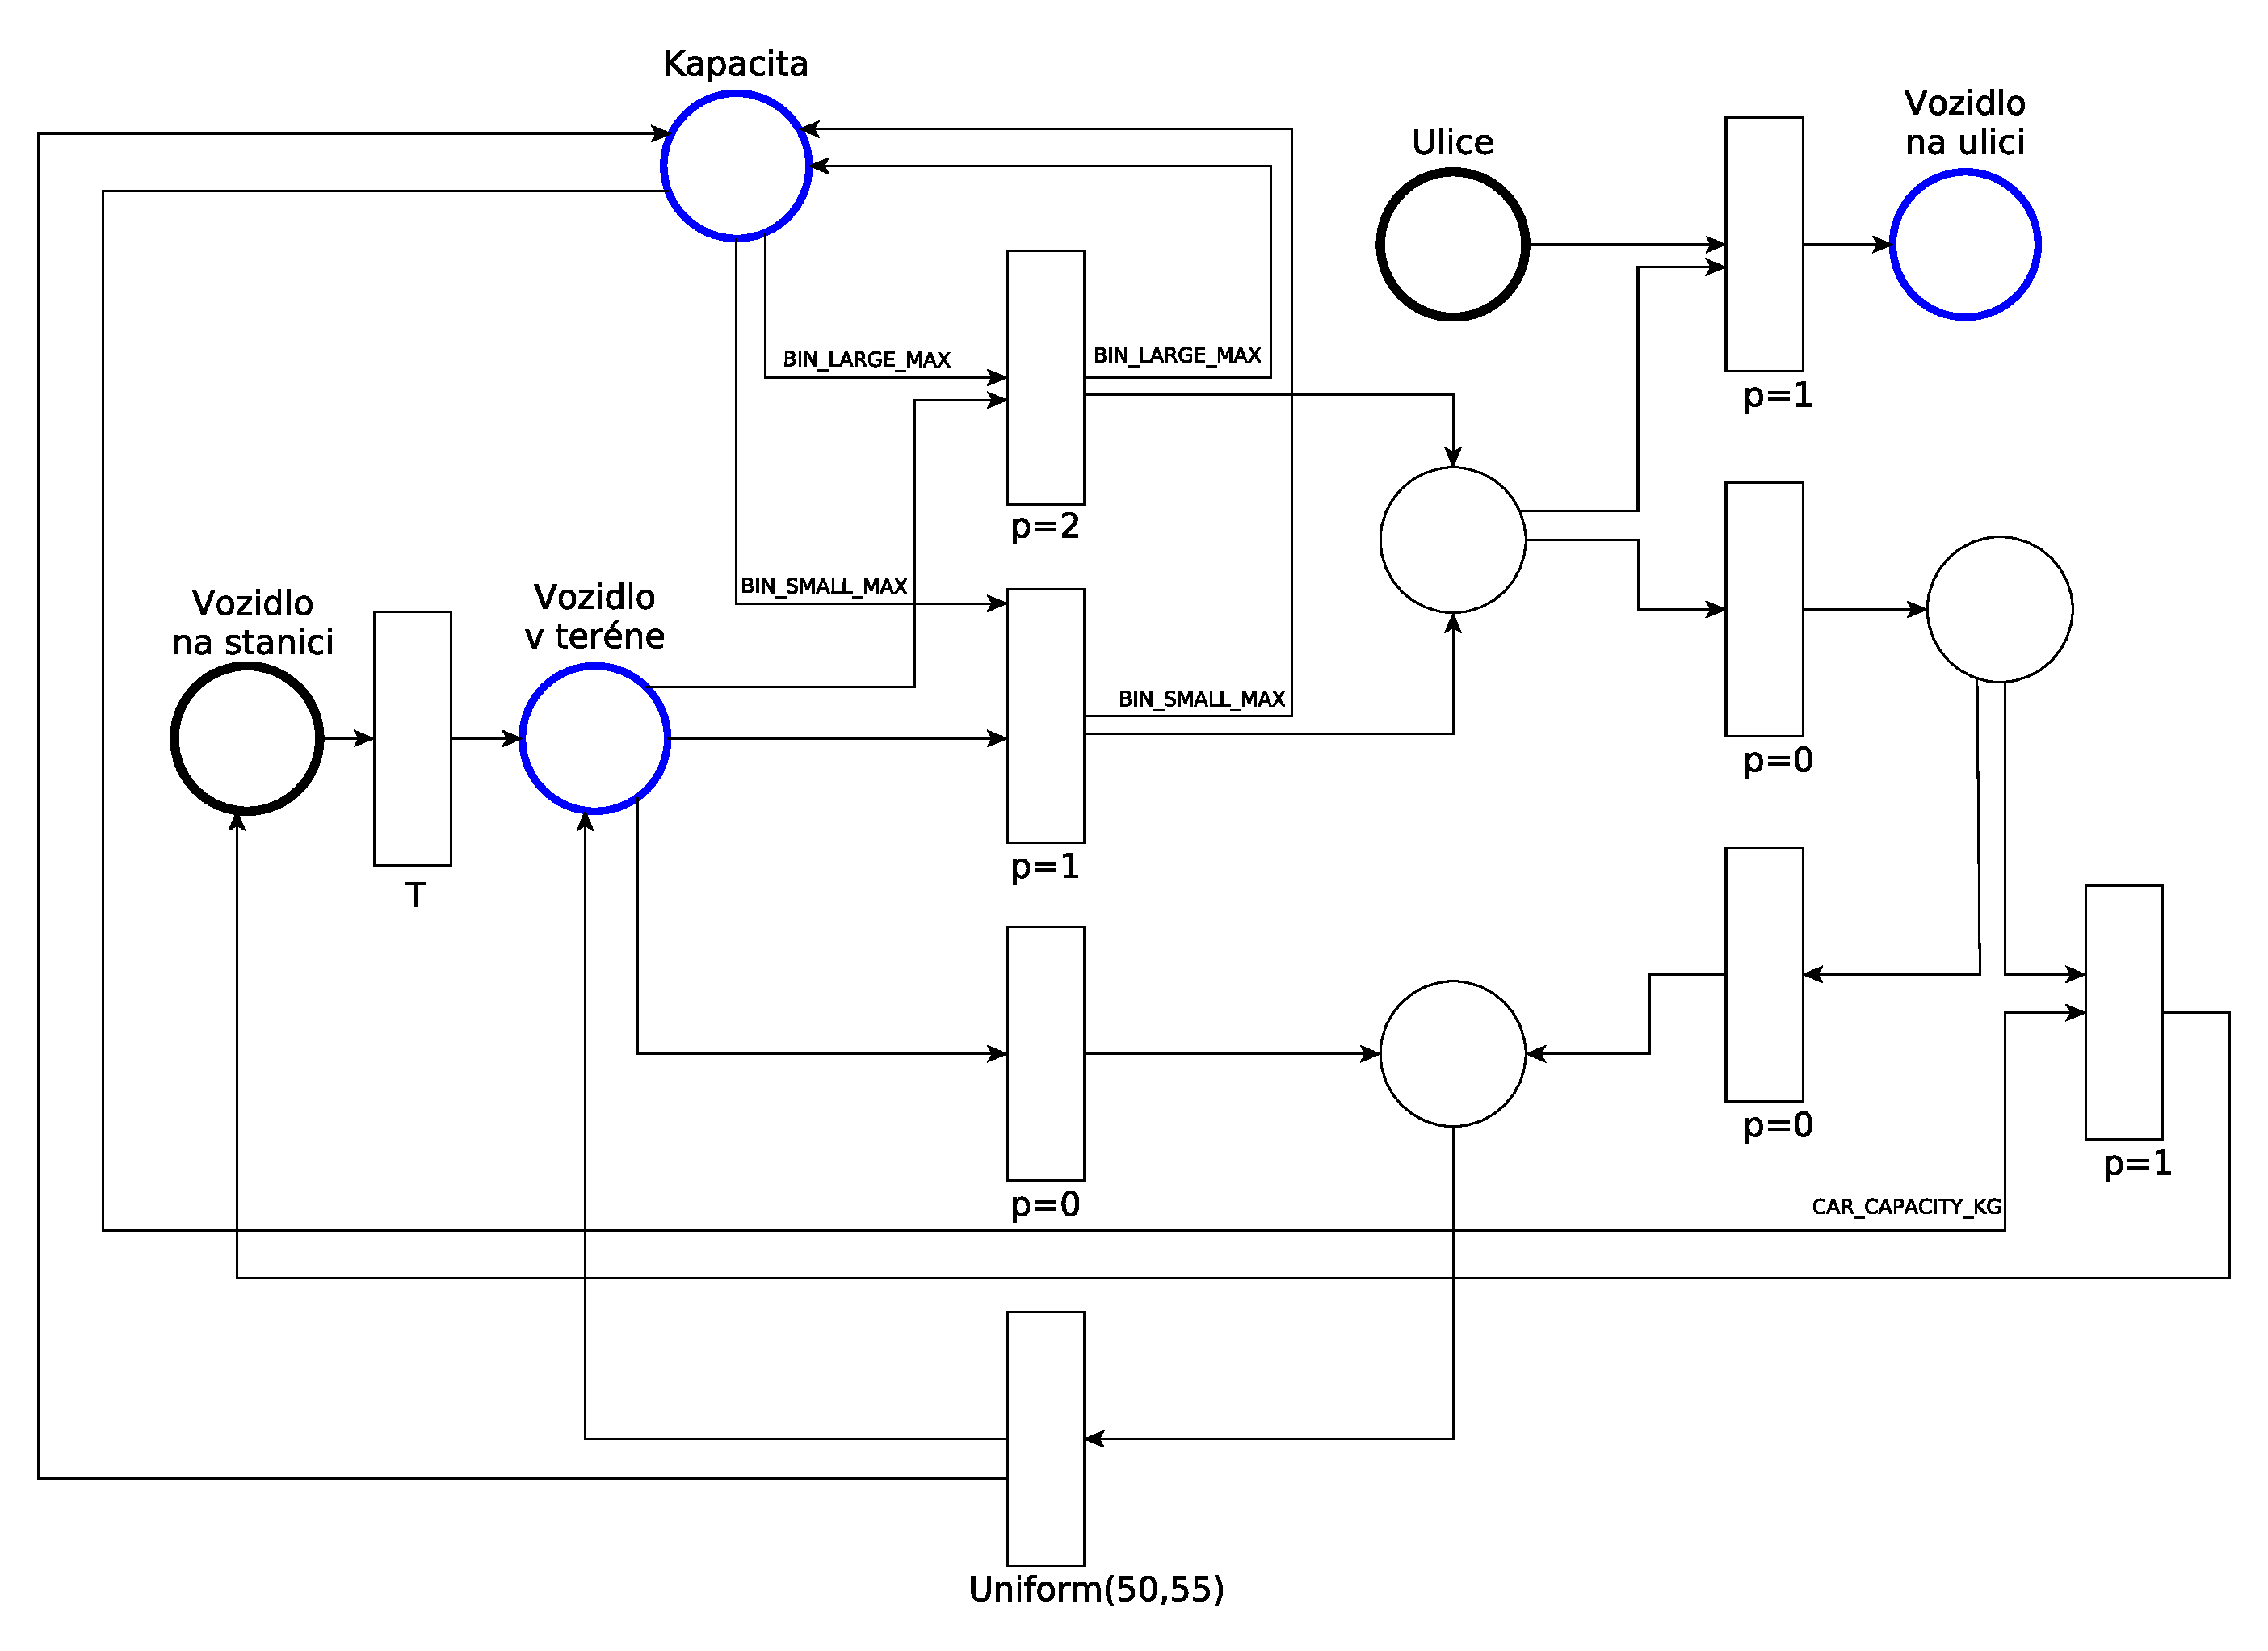
\includegraphics[scale=0.35]{../pn/pn-part1.eps}
    \caption{Petriho sieť (časť 1)}
    \label{PN-P1}
\end{figure}

\begin{figure}[H]
    \center
    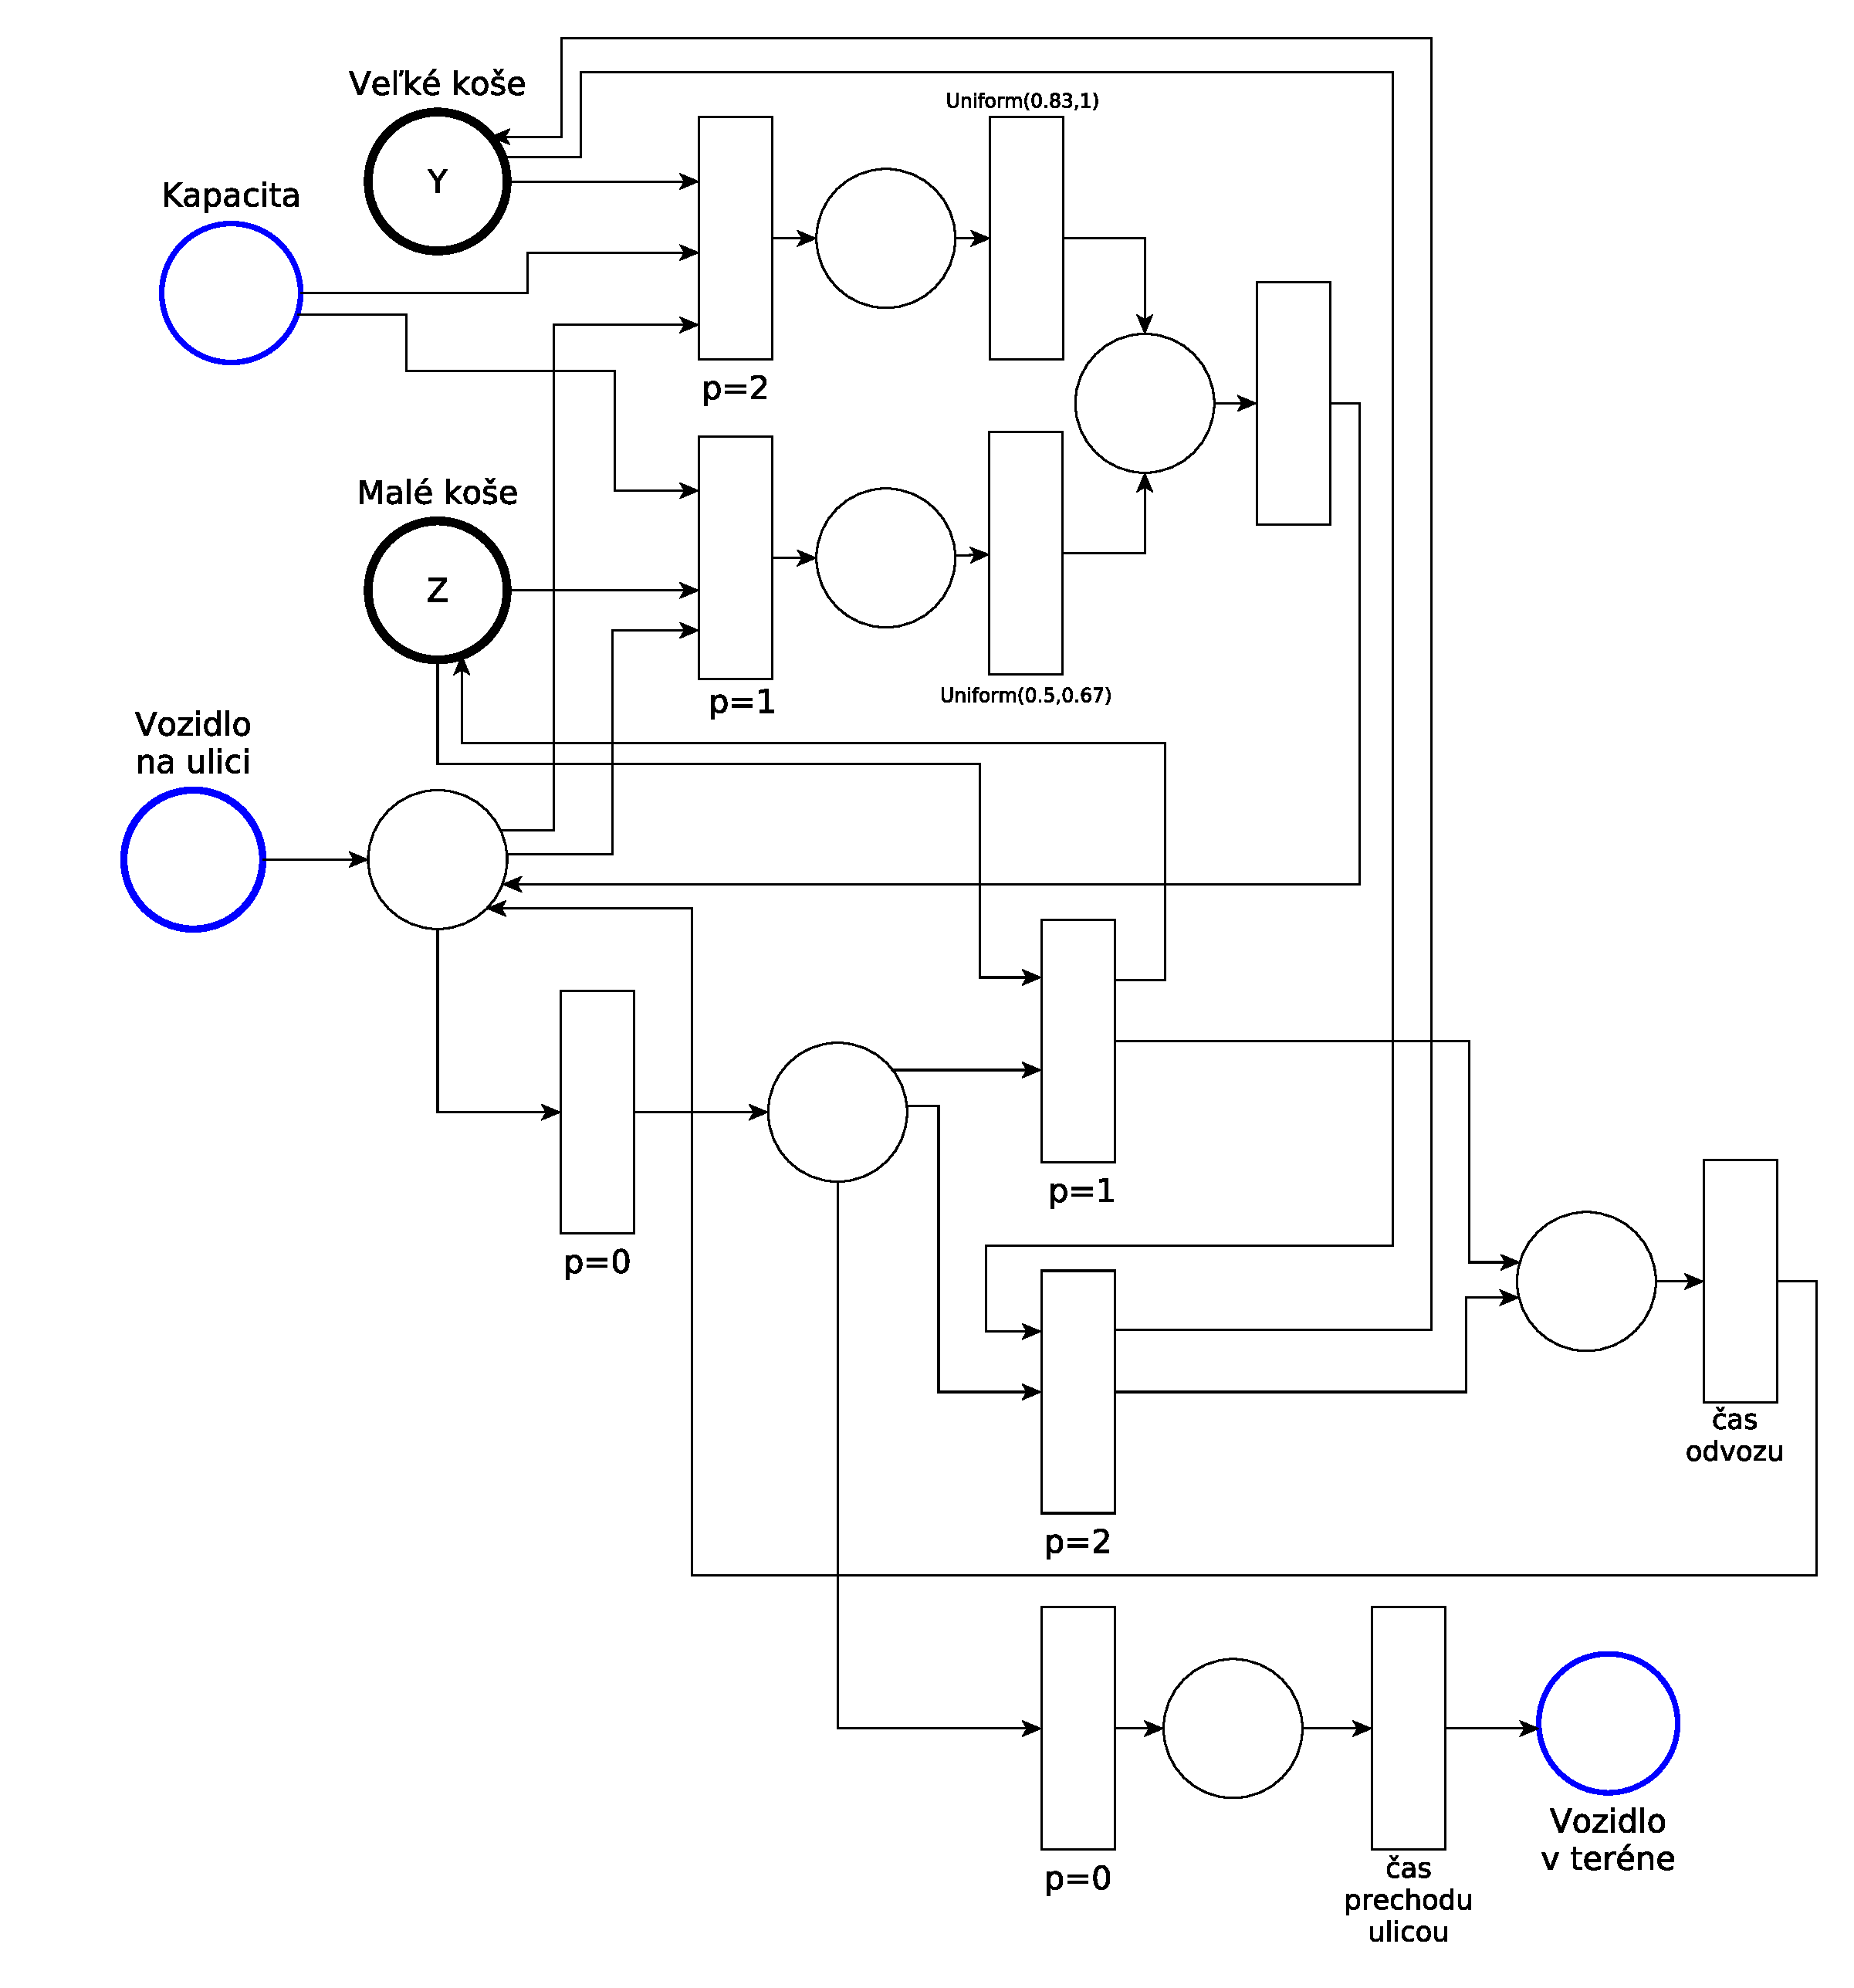
\includegraphics[scale=0.4]{../pn/pn-part2.eps}
    \caption{Petriho sieť (časť 2)}
    \label{PN-P2}
\end{figure}

\newpage %#########################################################################################

\makeatletter
\makeatother
\bibliographystyle{czechiso}
\begin{flushleft}
    \bibliography{quotation}
\end{flushleft}

\end{document} %###################################################################################


